% This document is a manually created, LaTeX version, of the original document at:
%      https://github.com/DP-3T/documents/blob/master/DP3T%20White%20Paper.pdf
% as captured on 2020-04-08.
%
% This version is to facilitate easier edits/contributions and collaboration.
%

\documentclass[10.8pt,a4paper]{article}
\usepackage[utf8]{inputenc}
\usepackage{amsmath}
\usepackage{amsfonts}
\usepackage{amssymb}
\usepackage{graphicx}
\usepackage{xcolor}
\usepackage[top=1.5in,bottom=1in, left=1in, right=1in]{geometry}
\usepackage{fancyhdr}
\pagestyle{fancy}
\fancyhf{}
\rhead{\thepage}
\renewcommand{\headrulewidth}{0pt}
\usepackage{setspace}
\usepackage{hyperref}
\hypersetup{
  colorlinks   = true,
  urlcolor     = blue,
  linkcolor    = blue,
}
\usepackage{float}
\fancypagestyle{specialfooter}{%
  \fancyhf{}
  \renewcommand\headrulewidth{0pt}
  \fancyfoot[R]{CC-BY 4.0}
}

\usepackage{helvet}
\renewcommand{\familydefault}{\sfdefault}
\setlength{\parindent}{0em}
\setlength{\parskip}{1em}

\begin{document}
%\thispagestyle{empty}
\thispagestyle{specialfooter}
\onehalfspace

\begin{center}{\bfseries\Large
Decentralized Privacy-Preserving\\
Proximity Tracing}\\[0.5cm]
 based on version: 8rd April 2020 -- non authoritative version \\

 \section*{Disclaimer/Provenance}

This document is a manually created, LaTeX version, of the original document at \url{https://github.com/DP-3T/documents/blob/master/DP3T\%20White\%20Paper.pdf} as 
as captured on 2020-04-08. As this document was only available as a PDF it was hard to collaborate in typical Open Source style.

This\emph{ non-authoritative, derived}, version is to facilitate easier edits/contributions and collaboration.

See \url{https://github.com/DP-3T/} for the correct versions.
\end{center}

\pagebreak
\begin{center}{\bfseries\Large

Decentralized Privacy-Preserving\\
Proximity Tracing}\\[0.5cm]
 based on version: 3rd April 2020 -- non authoritative version 

Contact the first author for the latest version.\\[1cm]
\textbf{EPFL} : Prof. Carmela Troncoso, Prof. Mathias Payer, Prof. Jean-Pierre\\
Hubaux, Prof. Marcel Salathé, Prof. James Larus, Prof. Edouard
Bugnion, Dr. Wouter Lueks, Theresa Stadler, Dr. Apostolos Pyrgelis, Dr.
Daniele Antonioli, Ludovic Barman, Sylvain Chatel

\textbf{ETHZ} : Prof. Kenneth Paterson, Prof. Srdjan Capkun, Prof. David Basin,
Dennis Jackson

\textbf{KU Leuven} : Prof. Bart Preneel, Prof. Nigel Smart, Dr. Dave Singelee,
Dr. Aysajan Abidin

\textbf{TU Delft} : Prof. Seda Guerses

\textbf{University College London} : Dr. Michael Veale

\textbf{CISPA} : Prof. Cas Cremers

\textbf{University of Oxford} : Dr. Reuben Binns

\textbf{TU Berlin / Fraunhofer HHI} : Prof. Thomas Wiegand

\textbf{University of Torino / ISI Foundation} :  Prof. Ciro Cattuto

\end{center}
\clearpage
\singlespace

\pagebreak

\section*{Disclaimer/Provenance}

This document is a manually created, LaTeX version, of the original document at \url{https://github.com/DP-3T/documents/blob/master/DP3T\%20White\%20Paper.pdf} as 
as captured on 2020-04-08. As this document was only available as a PDF it was hard to collaborate in typical Open Source style.

This\emph{ non-authoritative, derived}, version is to facilitate easier edits/contributions and collaboration.

See \url{https://github.com/DP-3T/} for the correct versions.

\pagebreak

\section*{Executive Summary}

This document proposes a system for secure and privacy-preserving proximity tracing  (aka contact tracing)  at large scale. This system provides a technological foundation to help slow the spread of the SARS-CoV-2 virus by simplifying and accelerating the process of notifying people who have been in contact with an infected person. The system design aims to minimise privacy and security risks for individuals and communities and guarantee the highest level of data protection.

The goal of proximity tracing is to determine who has been in close physical proximity to an infected person, without revealing the contact’s identity or where this contact occurred. To achieve this goal, users continually run a smartphone app that broadcasts an ephemeral, pseudo-random ID representing the user and also record pseudo-random IDs observed from smartphones in close proximity. Whenever a patient is diagnosed for COVID-19, she can upload some anonymous data from her phone to a central server. This step should only be done with the approval of a health authority and the explicit permission of the individual. Before, all data remains exclusively on the user’s phone. Other instances of the app can use the anonymous data from the server to locally compute whether the app’s user was in physical proximity to an infected person and the risk that an encounter led to a propagation of the virus. In case the app detects a high risk, it will inform the user. Additionally, the system enables users to voluntarily provide information to epidemiologists, in a privacy-preserving manner, to enable studies of the evolution of the disease and to assist in finding better policies to prevent further infections.

The system provides the following security and privacy protections:

\begin{description}
\item[Ensures data minimization] The central server only observes anonymous identifiers of infected people without any proximity information; health authorities learn no information (beyond when a user manually reaches out to them after being notified);
and the epidemiologists obtain an anonymized proximity graph with minimal information.
\item[Prevents abuse of data] As the different entities in the system receive the minimum amount of information tailored to their requirements, none of them can abuse the data for other purposes, nor can they be coerced or subpoenaed to make other data available.
\item[Prevents tracking of non-infected users] No entity, including the backend, can track non-infected users based on broadcasted ephemeral identifiers.
\item[Graceful dismantling] The system will organically dismantle itself after the end of the epidemic. Infected patients will stop uploading their data to the central server, and people will stop using the app. Data on the server is removed after 14 days.
\end{description}

We are publishing this document to seek feedback from a broad audience on the high-level design, its security and privacy properties, and the functionality it offers; so that further protection mechanisms can be added if weaknesses are identified. In particular, we seek feedback on the unlinkable design, as it presents overall better privacy properties. This document is accompanied by an overview of the data protection compliance of the design.

\clearpage
\section*{Changelog}


7 April 2020

General:

\begin{itemize}
\item Numbered sections for easier referencing.
Goals and requirements:
\item Clarify app sends notification (Section 2)
\item Add detail about most relevant information for epidemiological analysis (Section
1.1)
\item Add non-goals of the system (response issue \#33, Section 1.1)
\end{itemize}

Previous design (renamed:   Low-cost decentralized proximity tracing,  in Section 2)

\begin{itemize}
\item Clarification on data sent to epidemiologists (Section 2, Epidemiologists)
\item Slight tweak to design: send the day  t  explicitly when reporting an infected key
$SK_t$  , be clear that $ t$  is a global rather than local counter (Section 2, Setup) 
\item Added second operation point in scalability (Section 2, Scalability)
\item Interoperability: added possibility of mobile network carrier, and changed hard
coded to config file (response issue \#26, Section 2, Interoperability)
\end{itemize}

Added alternative design  ( Unlinkable decentralized proximity tracing , in Section 3)

\begin{itemize}
\item Added a new design that: prevents broadcast of seeds, provides unlinkability between EphIDs, enables users to redact EphIDs that they do not want published
\end{itemize}

Security and Privacy analysis
\begin{itemize}
\item Clarified that no notification is automatically sent to the health authority (response
issue \#52)
\item Added introduction to threat model (response issue \#47, Section 4.1)
\item Removed redacting mitigation from low-cost design (not possible due to hash
chain)
\item Added replay attack to create fake contacts on low-cost design (Section 4.3)
\item Added security and privacy analysis of unlinkable design (Sections 4.2 and 4.3)
\item Added comparison with both unlinkable design and low-cost design in the table
(Section 5.4)
\end{itemize}

\section{Goals and Requirements}
\subsection{System Goals}
\textbf{1) Enable quick notification of contact persons at risk and give guidance on next
steps}\\
In Switzerland, the proximity tracing (also known as contact tracing) process is legally
anchored in the \href{http://www.rki.de}{\underline{Infection Protection Act}} and is carried out by the health authorities. Other countries have similar laws. The multi-stage procedure is \textbf{\textit{time-consuming}} and requires a \textbf{\textit{large number of trained personnel}}. Under the current process, an employee of the health authorities conducts an in-person interview with an infected person to trace her or his contact history and identify other people who are likely to have contracted a disease. However, this process is slow and the \textbf{\textit{results incomplete}} as usually patients are \textbf{\textit{often unable to recall without gaps all contacts over a period of days}}. Furthermore, \textbf{\textit{random contacts}} (e.g., seat neighbours in public transport) \textbf{\textit{cannot be identified}}  and alerted.

Fortunately, most adults carry smartphones throughout the day, which opens the possibility
of an app that can aid health authorities in their efforts to quickly and precisely notify all individuals who have been in close proximity to an infected person during an infectious period. We call the process that enables the health authority to learn whom to notify proximity tracing.

\textbf{2) Enable epidemiologists to analyse the spread of SARS-CoV-2}\\
Currently, there is a \textbf{\textit{lack of detailed data}} on the spread of SARS-CoV-2. Epidemiologists
are trying to understand the key factors in the spread of the virus. More precise and timely
data would enable epidemiologists to improve their recommendations to policy makers and
health authorities about the most important and effective measures during the containment
phase of this and future pandemics.

The application should provide users with the possibility to \textbf{\textit{voluntarily share data with epidemiologists}} and research groups to enable these groups to reconstruct the interaction graph among infected and at-risk users (referred to as a \textbf{\textit{proximity graph}}). The information most relevant to the analysis carried out by epidemiologists is  relative timing information : at which phase of the infection did a contact occur?

\subsection{Out of scope goals}

The app does not aim to provide these functionalities:

\begin{description}
\item[Tracking infected patients ] once infected patients report themselves, the app does
not attempt to track them, nor does it provide a mechanism to ensure that they comply with medical orders. Recall that the goal of the app is to avoid asymptomatic users unknowingly spreading a disease. Diagnosed users are assumed to be responsible and take precautions if necessary to go into public, for instance to a doctor appointment. We do not attempt to detect or prevent misbehavior. The reason being that the gain in utility (one irresponsible person being under control) does not justify the loss of privacy for other well-behaved infected users. Moreover, this is not a location-tracking app and cannot determine when a user is “in public.”
\item[Finding hotspots or infected users’ trajectories ] the app does not attempt to identify locations that have a concentration of infected people. This is a design decision. We limit the purpose of the application to the two goals specified above, which enable us to collect and process very little data. In particular it avoids collecting location data, which is highly sensitive and very difficult to publish in a privacy-preserving way.
\end{description}

\subsection{System requirements}

\textbf{1) Functional requirements}

To achieve the system goals outlined above, the application must fulfill these functional
requirements:
\begin{itemize}\itemsep0pt
\item \textbf{Completeness}:  The contact history is \textbf{comprehensive}  regarding contact events.
\item \textbf{Precision}:  Reported contact events \textbf{must reflect}  actual physical proximity
\item \textbf{Integrity}: Contact events corresponding to at-risk parties are \textbf{authentic} , i.e., users cannot fake contact events.
\item \textbf{Confidentiality}:  A malicious actor cannot access the contact history of a user
\item \textbf{Notification}:  At-risk individuals can be informed
\end{itemize}
\textbf{2) Respect and preserve digital right to privacy of individuals}\\
It is of paramount importance that any digital solution to enhance proximity tracing \textbf{respects the privacy of individual users and communities} and \textbf{complies with relevant data protection guidelines} such as the European General Data Protection Regulation ( see \href{http://edpb.europa.eu}{\underline{EDPB Statement on GDPR and COVID-19}}) . The GDPR does not stop the use of data for public health, particularly in times of crisis, but it still imposes a binding obligation to ensure that 'only personal data which are necessary for each specific purpose of the processing are processed' (art 25). It is therefore a legal requirement to consider, particularly in the creation of systems with major implications for rights and freedoms, whether such a system could be technically designed to use and retain less data while achieving the same effect. To this end, an application must minimize the amount of data collected and processed to avoid risks for individuals and communities, and it should reveal only the minimum information truly needed to each authorized entity.

Furthermore, a common concern with systems like these is that the data and infrastructure
might be used beyond its originally intended purpose. Data protection law supports the
overarching principle of ‘purpose limitation’ — precluding the widening of purposes after the crisis through technical limitations. Such assurances will likely be important to achieve the necessary level of adoption in each country and across Europe, by providing citizens with the confidence and trust that their personal data is protected and used appropriately and carefully. Only applications that do not violate a user’s privacy \textbf{by design} will be widely accepted.

The system should provide the following guarantees:
\begin{itemize}\itemsep0pt
\item \textbf{Data use}: Data collection and use should be limited to the purpose of the data collection: proximity tracing and proximity graph reconstruction. This implies that the design should avoid collecting and using any data, such as for example geolocation
data, that is not directly related to the task of detecting a close contact between two
individuals.
\item \textbf{Controlled inference}: Inferences about individuals and communities, such as
information about social interactions or medical diagnosis, should be controlled to
avoid unintended information leakage. Each authorised entity should only be able
learn the information strictly necessary to fulfill the functional requirement.
\item \textbf{Protect identities}: The system should collect, store, and use anonymous or
pseudonymous data that is not directly linkable to an individual’s identity where
possible.
\item \textbf{Erasure}: The system should respect best practices in terms of data retention periods and delete any data that is not relevant.
\end{itemize}
\textbf{3) Fulfill the scalability requirements posed by a global pandemic}\\
SARS-CoV-2 is rapidly spreading across the globe due to the free movement of people
across national borders and continents. As a core principle of free democracies, after the
current confinement measures end, free movement should resume. Proximity tracing must
support free movement across borders and scale to the world’s population.

The system should give the following guarantees:
\begin{itemize}\itemsep0pt
\item \textbf{Scalability}:  The system scales to billions of users.
\item \textbf{Interoperability}:  The system works across borders and health authorities.
\end{itemize}
\textbf{4) Feasibility under current technical constraints}\\
There is an urgency to not only design but \textbf{\textit{implement}} a digital system that simplifies and accelerates proximity tracing in the near future. This mandates a system design that is \textbf{\textit{mindful of the technical constraints}}  posed by currently available technologies.
\begin{itemize}\itemsep0pt
\item \textbf{No reliance on new breakthroughs}: The system should, as far as possible, only
use techniques and methods readily available at the time of development and avoid
relying on new breakthroughs in areas such as GPS localisation or Bluetooth
distance measurements.
\item \textbf{Widely available hardware} : The goal of high adoption of proximity tracing can only
be achieved if both server- and client-side applications can run on widely available
smartphones and server hardware
\end{itemize}
\clearpage


\section{Design 1: Low-cost Decentralized proximity tracing}
We propose a privacy-friendly, decentralized solution that reveals minimal information to the backend server. To facilitate proximity tracing, smartphones locally generate ephemeral bluetooth identifiers (\texttt{EphIDs}) and broadcast them. Other smartphones observe these \texttt{EphIDs} and store them together with the duration and a coarse indication of time (e.g., “The morning of April 2”). See Figure \ref{AA}.

The proximity tracing process is supported by a backend server that shares infection
information with the app running on each phone. This backend server is trusted to not add or remove information shared by the users and to be available. However, it is untrusted with regards to privacy (\textit{i.e., collecting and processing of personal data}). In other words, the privacy of the users in the system does not depend on the actions of this server. Even if the server is compromised or seized, privacy remains intact.

When patients are diagnosed with SARS-CoV-2, they will be authorized by national health
authorities to publish information. Then, they will instruct their phones to upload to the
backend a compact representation of their \texttt{EphIDs} for the infectious period. The backend stores these \textit{compact representations}. Other smartphones periodically query the backend for this information and reconstruct the corresponding \texttt{EphIDs} of infected patients locally. If the smartphone has stored a record of any of these infected \texttt{EphIDs}, then the smartphone’s user has been in contact with an infected person and the smartphone computes the owner’s risk score. If this score is above the threshold the smartphone initiates a notification process.
\begin{figure}[H]
\centering
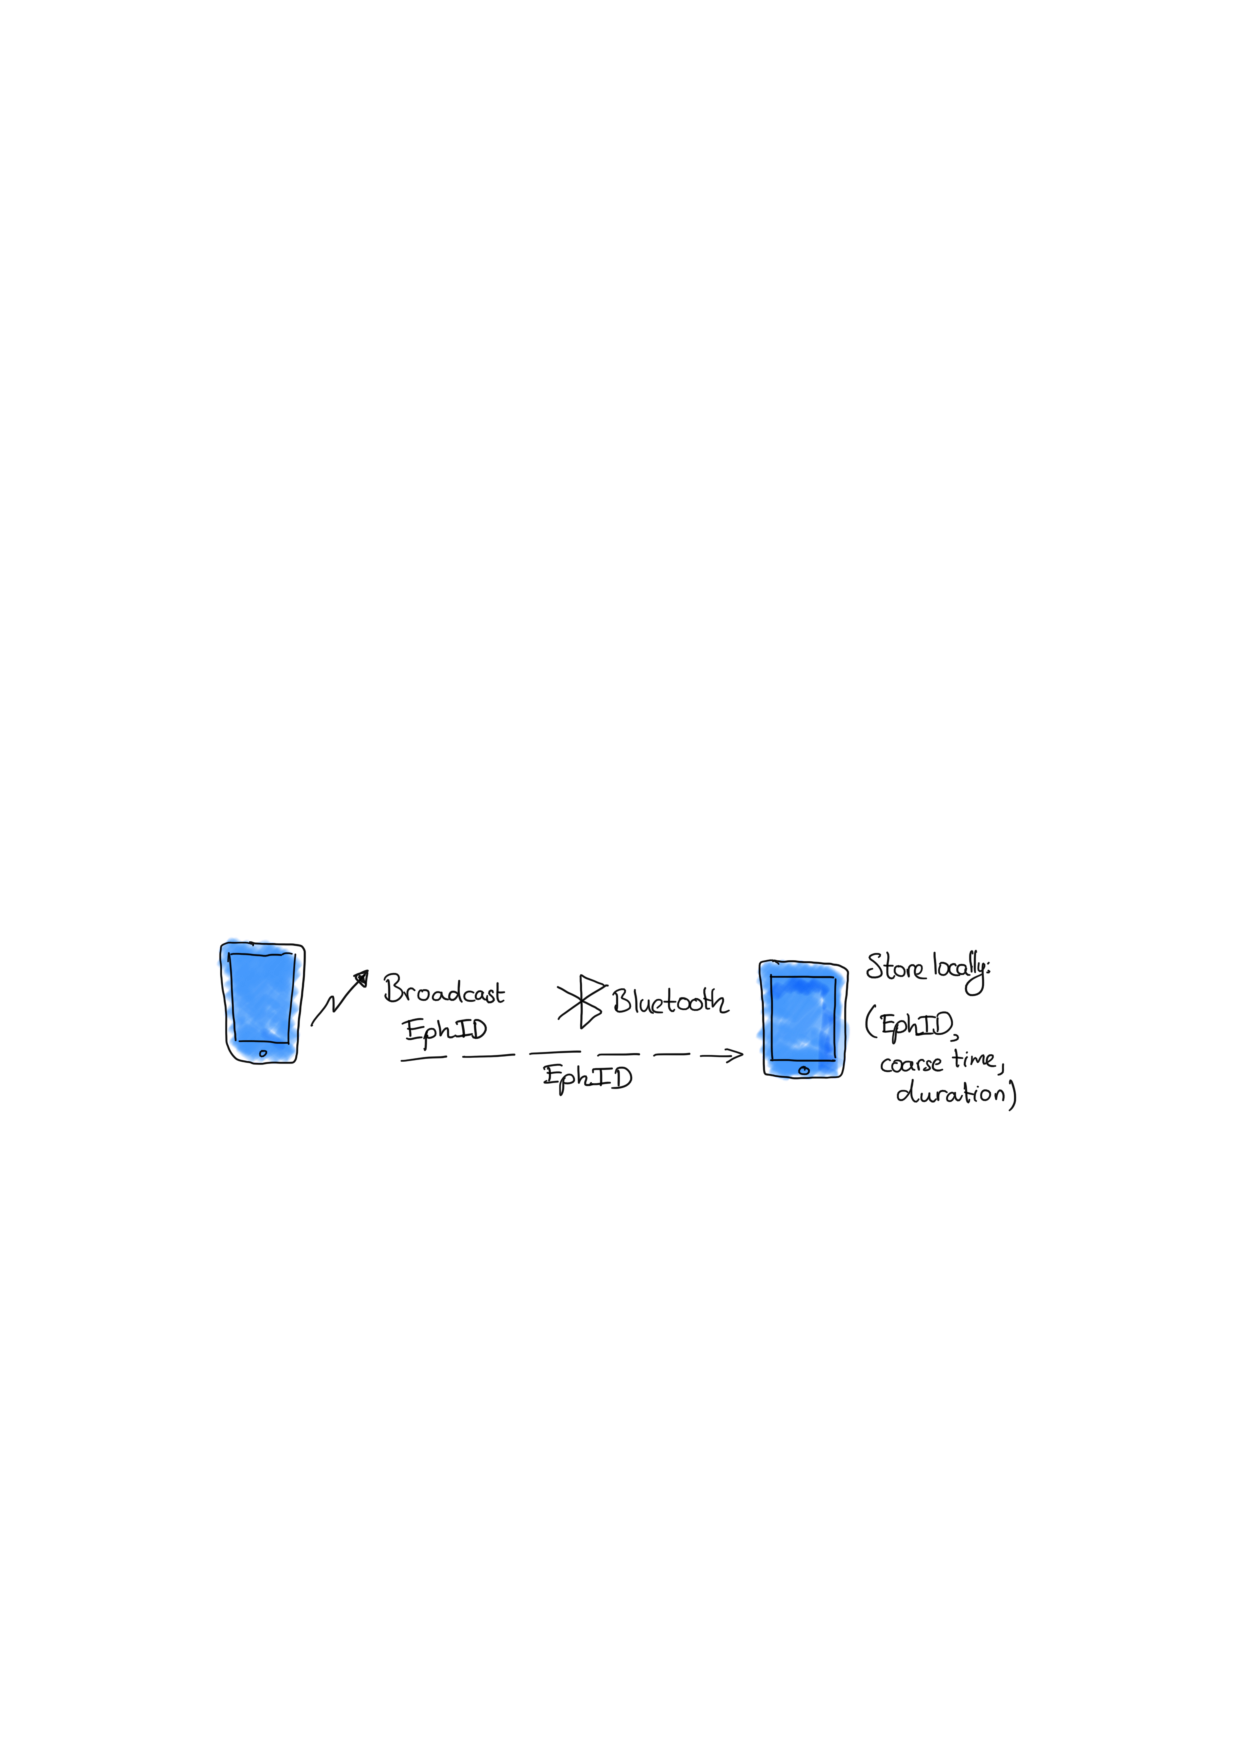
\includegraphics[scale=0.6]{fig/AA}
\caption{Processing and storing of observed \texttt{EphIDs}.}
\label{AA}
\end{figure}

\subsection{Setup}

\textbf{Generating a key} Let $t$ be the current day (e.g., indexed by some fixed staring point for the system). 
Smartphones generate a random initial daily key $SK_0$. 


\subsection{Creating ephemeral IDs ( EphIDs )}


\texttt{\textit{EphID}} Constraints. Given the completeness requirement, it is necessary that smartphones can observe and record as many \texttt{EphIDs} as possible. This precludes the use of connection-based communication between smartphones, as establishing connections limits the amount of exchanges of \texttt{EphIDs}. Instead, we rely on Bluetooth Low Energy beacons. These beacons’ payload is 16 bytes, which technically limits the size of our system’s \texttt{EphIDs}.

\texttt{\textit{EphID} Generation}. Smartphones generate a stream of secret day keys $\texttt{SK}_\texttt{t}$ , by computing

\[\texttt{SK}_\texttt{t}  = \texttt{H}(\texttt{SK}_\texttt{t} - 1) ,\]

where \texttt{H} is a cryptographic hash function. The smartphone will use the secret key $\texttt{SK}_\texttt{t}$ during day \texttt{t}  to generate \texttt{EphIDs}.

Smartphones locally generate $\texttt{EphID}_\texttt{i}$s to use during day \texttt{t} as follows. Let \texttt{t} be the current day, and n the number of distinct \texttt{EphIDs} we must generate for that day. Then the smartphone computes

\[\texttt{EphID}_1\  \vert\ \vert\ \ldots\ \vert\ \vert\ \texttt{EphID}_\texttt{n}\ =\ \texttt{PRG} (\ \texttt{PRF}(\texttt{SK}_\texttt{t} ,\ “\texttt{broadcast key}”)\ )\]


where \texttt{PRF} is a pseudo-random function (e.g., HMAC-SHA256), “\texttt{broadcast key}” is a fixed and public string, and PRG is a stream cipher (e.g., AES in counter mode) producing \texttt{n} $\ast$ \texttt{16} bytes, which we split into 16-byte chunks to obtain the \texttt{n} ephemeral Bluetooth identifiers \texttt{EphID} of the day.

Smartphones pick \textbf{a random order} in which to broadcast the \texttt{EphID} during the day. Each \texttt{EphID} is broadcast for (24 $\ast$ 60)/\texttt{n}  minutes
\subsection{Local storage of observed \texttt{EphIDs}}

Smartphones locally store each observed \texttt{EphID} together with the corresponding proximity, duration, and other auxiliary data, and a coarse time indication (e.g., “The morning of April 2”). See Figure \ref{AA}.

Local storage of observed $EphID$s and keys $SK_t$

Smartphones locally store each observed $EphID$ together with the corresponding proximity, duration, and other auxiliary data, and a coarse time indication (e.g., “The morning of April 2”). See Figure \ref{AA}. Besides, each device stores the keys $SK_t$ it generated during the past 14 days. This parameter, which defines the maximum period for which any data (both observed and generated $EphID$s) are stored on the device is a system parameter and is determined by guidance from health authorities.

\subsection{Decentralized proximity tracing}
The decentralized proximity tracing process requires the participation of infected patient’s smartphones, all other smartphones, the backend, and the health authority. The backend acts \textbf{solely}  as a communication platform and does not perform any processing.

The health authority is responsible for informing patients of (positive) test results, authorizing uploads from phones to the backend, and determining the contagious window, i.e., during what time the patient was contagious and might have infected others. Epidemiologists estimate that the contagious window starts 1 to 3 days before the onset of symptoms. The start of the contagious window determines for which time frame phones upload information.

For safety reasons, health authorities often notify patients by phone about positive test results. Therefore we propose that when administering the test, health authorities provide the patient with an inactive authorization code. If the test is positive, health authorities activate the authorization code, and contact the patient to inform them of the result and ask them to start the proximity tracing process.


Once the health authority triggers proximity tracing for an individual (Figure \ref{PT}, step 1), the patient instructs their phone to send to the backend the key $\texttt{SK}_\texttt{t}$ corresponding to the first day in which the app user was considered to be infectious (Figure \ref{PT}, step 2). Note that given the key $\texttt{SK}_\texttt{t}$ , everyone can compute all ephemeral identifiers \texttt{EphID} used by the infected patient starting from epoch $t$ by repeating the process described in “\texttt{EphID} generation” above.

After reporting their current $\texttt{SK}_\texttt{t}$, the smartphone of the infected patient picks a new completely random key

Periodically, the backend sends the $\texttt{SK}_\texttt{t}$ of infected patients to all other smartphones in the system (Figure \ref{PT}, step 3). If an update is needed, it can also send to the smartphones the latest risk-scoring algorithm parameters provided by the health authority. Each smartphone uses this key to reconstruct the list of \texttt{EphIDs} of an infected person and checks if it has observed any of these \texttt{EphIDs} in the past (i.e., before the corresponding key $\texttt{SK}_\texttt{t}$ was published). If so, the smartphone owner may be at risk. The smartphone uses the risk-scoring algorithm with its local records corresponding to the infectious \texttt{EphID} , to determine the owner’s risk score. See Figure \ref{PT} step 4.

\begin{figure}[H]
\centering
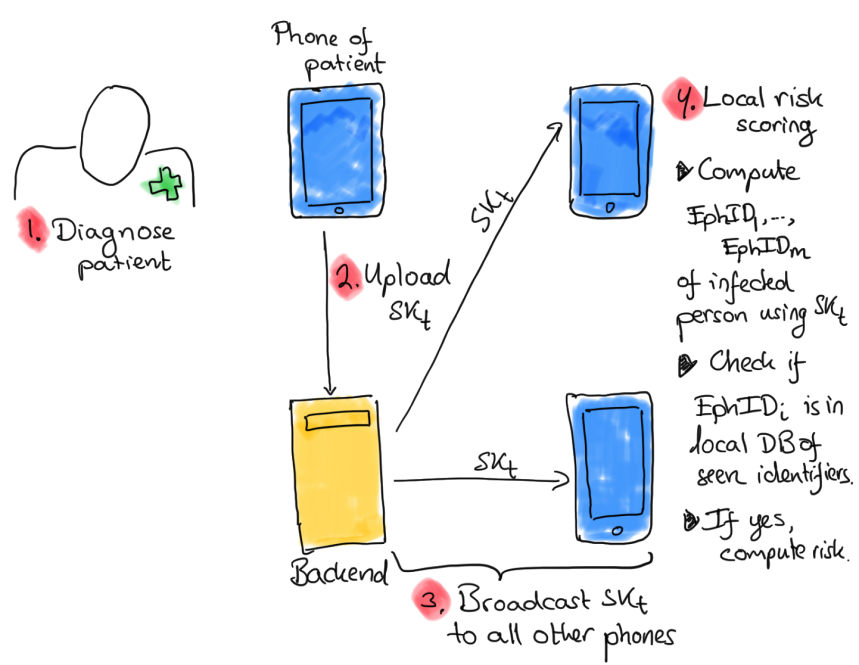
\includegraphics[scale=0.65]{fig/PT}
\caption{proximity tracing process.}
\label{PT}
\end{figure}
\subsection{Notification of Risk}
If the risk score computed in the previous step is below a threshold determined by the health authority, the smartphone does nothing. Otherwise, the smartphone displays a notification that the user has been in close proximity to an infected patient. The notification advises the user on what to do and where to find more information.
\subsection{Interoperability}
To enable interoperability between countries, the smartphone records the countries that a
user has visited. This can either happen automatically, in the background, based on GPS
location data or through a manual entry by the user (e.g., if GPS was not available or
inaccurate). To learn if a user has been in contact with an infected patient, the phone
regularly requests data (containing $\texttt{SK}_\texttt{t}$’s from infected users) from the backend services of all visited countries. The addresses of these backends can be hardcoded in the app. In case of a positive diagnosis, the smartphone uploads its own key $\texttt{SK}_\texttt{t}$ to the backends of all visited countries.

When the smartphone determines its owner has a high risk score, the smartphone contacts
its local health authority as if it was not roaming.

\subsection{Sharing data with epidemiologists}

When installing the app, users are asked if they want to opt-in to data sharing with epidemiologists. The data sharing is strictly limited to cases where there has been a contact with an infected person. No data is shared if there has never been a contact to an infected person. However, if users opt-in, the app will regularly (e.g., every day) upload fixed-size dummy data to the epidemiologists to defeat traffic analysis.

After a patient receives a notification that they are at risk, the app again prompts users to confirm their permission to share data with epidemiologists. If permission is given, at the next transmission time, the app sends to a selected research center  anonymous data about contact events the user had  with each infected individual o  ver the past period. In the low-cost design, infected individuals are represented by their keys  SK t. 

For each infected contact person, the user uploads a tuple consisting of a tag (boolean value) indicating if the user herself has been tested positive, the  SK t of the contact and metadata about the encounters. This metadata includes the number of encounters the user had with the infected individual and relative timing information about each encounter, i.e. during which phase of the infectious period the contacts occurred. Time is reported as the number of days  relative to the onset of symptoms (or an estimate in case there were no symptoms) , i  .e., relative to the corresponding day  t that the infected patient has reported to the health official. This information is enough for epidemiologists to build the first degree contact graph needed for their analysis.

No location or precise timing information about contact events will ever be shared. The data submitted enables epidemiologists to study the  proximity graph around an infected individual and to understand which circumstances and encounters led to an infection. However, it does not reveal any information about other encounters the user has had with non-infected people.

\subsection{Scalability}
The decentralized design scales very well. For each infected user, the backend needs to
store a 32 bytes key for the duration of the infectious window. Storage cost at the backend is therefore not a problem. Throughout the day, smartphones download the 32 byte keys of newly diagnosed patients. This data is static, and can therefore be effectively served through a content delivery network.

Smartphones download a very small amount of data every day. For 40.000 (approximately the cumulative of 5 european countries at their contagion peak) new infections per day, smartphones download 1.30 MB each day. For a smaller country such as Switzerland with 2.000 infections a day (at the contagion peak), smartphones need to download 66 kB each day. 

They require a few seconds of computation time to regenerate the ephemeral keys $EphID$ , and to check if they are included in the local list of observed  $EphID$s ..

\clearpage

\section{Design 2: Unlinkable decentralized proximity tracing}

In this section we present a variant of the low-cost design from the previous section that offers better privacy properties at the cost of larger volume of downloads to smartphones. In this design, there is no need to disseminate a public list of the seeds corresponding to infectious individuals. Instead, the ephemeral identifiers of infectious individuals are hashed and stored in a Cuckoo filter, which is then distributed to users of the system.

This design offers several advantages over the earlier proposal. It prevents malicious users from linking the ephemeral identifiers of infectious individuals, enables infected users to redact their identifiers corresponding to sensitive locations or times, and supports flexible time periods in which users are considered infectious.

\subsection{Setup}

No setup is needed.

\subsection{Generating ephemeral IDs}

Smartphones generate the ephemeral Bluetooth identifier  $EphID$ t for epoch $ t$ as follows.

The smartphone draws a random 32-byte per-epoch seed $ seed_t$  and sets: 

$EphID_t  = TRUNCATE128( H( seed_t  ) ) $

Where  $H$ is a cryptographic hash function, and  $TRUNCATE128$ truncates the output to 128 bits. Smartphones store the seeds corresponding to epochs in the last 14 days. They delete older seeds.

\subsection{Local storage of observed EphIDs}

For each observed  $EphID $ the smartphone stores contact events:

\begin{itemize}
\item The hashed identity $ H(EphID||t)$ , where $ H$  is a cryptographic hash function,
\item The proximity,
\item The duration,
\item Other auxiliary data,
\item And a coarse time indication (e.g., “The morning of April 2”).
\end{itemize}

We include the epoch  t in the hash to ensure that replaying an $EphID$ outside the epoch in which it was originally broadcast can never cause a fake at-risk event (regardless of whether the $EphID$ corresponds to a person who is later marked as infected).

\subsection{Decentralized proximity tracing}

When patients are diagnosed, they upload a representation of the $EphID$s produced by the smartphone during the infectious window. Unlike the initial, low-cost approach, the patient first has the option to  redact their identifiers, by choosing the set of epochs  $T$ for which the patient wants to reveal their identifiers. For example, the patient may want to exclude monday morning and friday night. The phone then uploads the set  ${(t, seed+_t)  }$ for all epochs  $t $ in  $T$.

Periodically (e.g., every 4 hours), the backend creates a new Cuckoo filter  F and for each
pair  (t, seed  )  uploaded by an infected patients it inserts t 

$TRUNCATE128(H(H(seed _t  )||t))$

into the Cuckoo filter  $F$ . It then sends this filter to all smartphones in the system.

Each smartphone uses this filter  $F$ to determine if its user has been in contact with an infected person. To this end, the phone takes all the recorded hashes and checks if they are included in the filter  $F$ . If so, the smartphone user may be at risk. The smartphone computes the user’s risk score by applying the risk-scoring algorithm to the local records corresponding to identifiers included in the filter  $F$ . Cuckoo filters have a low, but non-zero, probability of false positives, that is reporting that they contain an element that was not in the input set. In order to avoid unnecessarily alarming users, we select the parameters of the Cuckoo filter such that false positives are highly unlikely to occur even with heavy usage of the system over a number of years.

The use of a Cuckoo filter hides the set of ephemeral identifiers belonging to infected individuals from the general public. The system uses a Cuckoo filter in conjunction with inputs that are obtained by truncation of cryptographic hashes of random values (the seeds). The inputs to the filter are sparse amongst the set of all possible inputs (128-bit strings). These two factors makes enumeration attacks against the filter an unattractive attack vector for adversaries, while still making it possible for users who have observed particular ephemeral Bluetooth identifiers to check for their inclusion in the filter. Attacks that attempt to reverse the filter and directly recover inputs from values held in the filter do not result in exposure of ephemeral IDs because of the extra layer of hashing that is performed on ephemeral IDs before entering them into the filter.

\subsection{Notification of risk and interoperability}

Same as the low-cost approach.

\subsection{Sharing data with epidemiologists}

\emph{Note: we are actively discussing with epidemiologists if the data provided by this design is sufficient to achieve their objectives}

As in the low-cost design: users have to opt-in explicitly to share data with epidemiologists. This sharing is limited to cases where the user has been in contact with an infected person. If users opt-in, the app will regularly (e.g., every day) upload fixed-size dummy data to the epidemiologists to defeat traffic analysis.

After a patient receives a notification that they are at risk, the app prompts users to confirm their permission to share data with epidemiologists. If permission is given, at the next transmission time, the app sends  to a selected research center \emph{ anonymous and aggregated data} about contact events the user had with infected individuals.

The app sends to the server a tag (boolean value) indicating if the user herself has been tested positive, and a list of the  number of unique infected  EphIDs  observed during each day of the past 14 days.

As in the low-cost design: no location or precise timing information about contact events will ever be shared.

\subsection{Scalability}

This design requires more bandwidth and storage. The backend needs to store cuckoo filters containing the hashed identities of infected people during an infectious period. Smartphones regularly download new cuckoo filters containing the latest hashed identities of patients. This data is static, and can therefore be effectively served through a content delivery network. The computational cost on the phone is likely smaller, as phones only need to do one lookup per stored identifier per cuckoo filter sent by the backend.

Smartphones download a manageable amount of data every day. We assume that the contagious window of infected patients is on average 5 days. For 40.000 new infections per day (approximately the cumulative total of 5 European countries at their contagion peak) smartphones then need to download 110 MB each day. For a smaller country, such as Switzerland, with 2.000 infections a day (at contagion peak), smartphones need to download 5.5 MB each day (assuming a 14 day history). The computation time to check if the previously observed identifiers are contained in the new cuckoo filter is negligible.

\section{Security and privacy considerations}

\subsection{Threat model}

In this section we describe the potential attackers that we assume when carrying out our security and privacy analysis. For each of these attackers we describe their capabilities and what kind of risk they pose for the system. In the next section, we analyze the security and privacy of the system with respect to these adversaries.

\textbf{Regular user}. A typical user of the system that is assumed to be able to install and use the application by navigating its user interface (UI). They will exclusively look at information available via the app UI to infer private information about other users.

\textbf{Tech-savvy user} (Blackhat/Whitehat hacker, NGOs, Academic researchers, etc.) .
This user has access to the system via the mobile App. Can set up (BT, WiFi, and Mobile)
antennas to eavesdrop locally. Can decompile/modify the app. Can have access to the
backend source code.
\begin{itemize}\itemsep0pt
\item (Whitehat hacker) Will investigate the App code, the information in the phone, and will look at what information is exchanged with the server (using an antenna or software
installed on the phone, e.g., \href{http://www.haystack.mobi}{\underline{Lumen}}) or broadcast via Bluetooth (passive).
\item (Malicious) Can DOS the system (targeted or system-wide), deviate from protocols, and actively broadcast Bluetooth identifiers.
\end{itemize}
\textbf{Eavesdropper} (Internet Service Provider, Local System administrators, Bluetooth sniffer). Can observer network communication (i.e., source and destination of packages, payload, time) and/or Bluetooth BLE broadcast messages.
\begin{itemize}
\item  (Network adversary) Can use observed network traffic to determine the state of a
user (e.g., whether they are at-risk, infected, etc.)
\item (Local Bluetooth BLE Sniffer) Can observe local Bluetooth broadcasts (possibly with
a big antenna to cover a wider area) and try to trace people.
\end{itemize}
It should be noted however that in many instances, for individuals or companies to use data in this way, such as to collect data about passers-by to try and estimate their infection status based on the announced identifiers, will fall foul of a range of existing national and European laws around data protection, ePrivacy and computer misuse.

\textbf{Health authority}. Receives information about infected people as part of their normal operations to diagnose patients. The health authority learn information about at-risk people only when these at-risk people themselves reach out to the health authority (e.g., after receiving a notification from their app).

\textbf{Epidemiologists}. Receive and analyse data about interactions between infected and at-risk users. Epidemiologists and related research groups are not in direct contact with app users and data is shared with them on a voluntary basis. They are mainly interested in learning the proximity graph around an infected user but can combine background knowledge about individual users with the inferred graph data to learn more about infected and at-risk users.

\textbf{Backend}. Can access all data stored at the servers. Moreover, the backend can query data from the mobile app in the same way that it would do during normal operations (in our system, it can only send). They could also change the code of their backend software and the code of the mobile apps. We assume they will not modify the mobile app because doing so would be detectable. They can combine and correlate information, request information from apps, combine with other public information to learn (co-)location information of individuals.

\textbf{State-level adversary (Law enforcement, intelligence agencies)}. Has the combined
capabilities of the tech-savvy user and the eavesdropper. In addition, a state-level adversary can obtain subpoenas that give them the capabilities of the health authority, epidemiologists or the backend. Their goal is to obtain information about the population or to target particular individuals. They may be interested in past information, already stored in the system, or future information that will enable them to trace target individuals based on observed \texttt{EphIDs}.
\subsection{Privacy}

\subsubsection{Privacy Concerns}
\textbf{Global interaction graph}. The global interaction graph reflects the social relationships of all users in the system. A labelled edge indicates an interaction between two adjacent users at a specific time. Knowledge of this graph is not necessary for proximity tracing nor for analyzing the spread of SARS-CoV-2. Therefore, \textit{no party} needs to learn the global interaction graph. Only the relevant subset of this graph, such as for example the proximity graph (below), should be revealed to the authorised entities.

\textbf{Proximity graph}. The proximity graph is a subset of the global interaction graph. It encodes contacts between infected users and others individuals. Every edge is adjacent to at least one infected patient. Edges can be labeled with coarse-grained timing information (e.g., “contact on the 4th of April”). This information is \textit{essential for epidemiologists} but not for any other party in the system.

\textbf{Infected individuals}. Only the individuals themselves, and the health authority, need to know that they are infected with SARS-CoV-2. No other parties in the system need to learn this information. In particular, infected users do not need to know which of the individuals they have been in contact with are infected.

\textbf{At-risk individuals}. At-risk individuals are people that have recently been in contact with somebody who has been infected with SARS-CoV-2. At-risk individuals need to know that they are at risk so that they can take appropriate measures. The health authority needs to know who is at risk so that they can notify them. No other parties in the system need to know this information.

\textbf{Location traceability}. To perform proximity tracing or to analyze the virus’ spread, location traces are not required, e.g. GPS coordinates. Therefore, no party in the system needs to have access to them, or be able to easily trace individuals based on the Bluetooth signals that the apps broadcast.

\subsubsection{Privacy Analysis of low-cost design}

\textbf{Interaction graph}. The system does not reveal any information about the interaction between two users to any entity other than the two users themselves. The \texttt{EphIDs} revealed by infected users do not allow any inference about the people they have been in contact with. The system thus prevents any one party from learning the interaction graph.

\textbf{Proximity graph}. By construction, the proximity graph (containing interactions between infected patients and other users) is only revealed to epidemiologists, with the specific, separate consent of a user, and not to any other party.

\textbf{Location traceability}. The \texttt{EphIDs} of all users are perfectly unlinkable, and only the smartphone that generated them knows the corresponding keys $\texttt{SK}_\texttt{t}$. When the phone’s owner is diagnosed with SARS-Cov-2, the phone publishes to the backend the key $\texttt{SK}_\texttt{t}$ corresponding to the first infectious day. After disclosing this information, the phone will generate a new key at random. Given this key $\texttt{SK}_\texttt{t}$, all corresponding \texttt{EphIDs} of the infected person are linkable during the infectious period.

As a result, tech-savvy users, eavesdroppers, and state-level adversaries with strategically placed Bluetooth receivers and recording devices can track infected patients during the (earlier) window in which the identifiers broadcasted via Bluetooth are linkable. The app’s Bluetooth broadcasts of non-infected people and infected people outside the infectious window remain unlinkable.

\textbf{At-risk individuals}. The keys revealed to the server by infected people are independent of their contacts, i.e., the people they interacted with. They therefore do not give any information about people at risk.

Smartphones locally compute at-risk status. The smartphone then relays this at-risk status to the health authority so that the health authority can contact the phone’s user. The health authority therefore learns who is at risk.

If the user consents, the smartphone uploads anonymized data about the user’s encounters
with infected individuals to epidemiologists. However, the information shared does not
include any pseudonyms or anonymous identifiers and does not allow linking contact events
to identities. Epidemiologists therefore cannot learn who is at risk, but they can study the spread of the virus through the proximity graph.

\textbf{Infected individuals}. Any proximity tracing mechanism that informs a user that he/she has been in contact with an infected person inherently reveals a piece of information to the person at risk: one of the people they interacted with has been infected. For the purpose of this analysis we will divide these people in three categories: 
\begin{itemize}\itemsep0pt
\item[-] \textit{Close individuals}: Family, friends, or colleagues with whom the at-risk individual spends long periods of time. If these people are infected, they will inform the at-risk user personally about their infection if they have spent time together. It is common practice that the authorities ask COVID-19 patients to notify any contact person at
risk they remember.
\item[-] \textit{Routine-sharing individuals}: People who share an activity with the at-risk individual such as riding a bus every day, supermarket tellers, etc. Infected individuals in this group will likely not remember having been in contact with them and therefore will not (and can not) notify the at-risk individual.
\item[-] \textit{Anonymous individuals}: People that the user sees sporadically. These people cannot be re-identified as their identities are unknown to the at-risk individual. They are therefore out of the scope for this analysis.
\end{itemize}
As close individuals will reveal themselves, there is no extra information that an at-risk
individual can gain about the infection status of this group by exploiting the app. Anonymous infected persons cannot be identified, so their privacy is also not at stake. In the remainder of this analysis we thus focus on routine-sharing individuals.

First, and foremost, the app in normal operation does not reveal to users anything about the \texttt{EphIDs} downloaded from the backend. Therefore, a curious user, who only uses the standard interface of the app, cannot learn who is infected. As this user does not perform further actions, they cannot obtain any further information about who is infected other than the information provided to them through app notifications, health officials, or by infected individuals themselves.

On the other end, a proactive tech-savvy person can abuse \textbf{\textit{any}} proximity tracing mechanism to narrow down the group of individuals they have been in contact with to infected individuals. To do so they must, 1) they keep a detailed log of who they saw when. 2) they register many accounts in the proximity tracing system, and use each account for proximity tracing during a short time window. When one of these accounts is notified, the attacker can link the account identifier back to the time-window in which the contact with an infected individual occurred. The attacker can correlate this information with the detailed log to narrow down who in their list of contacts is now infected. This attack \textbf{\textit{is inherent to any proximity-based system notification system}}, as the adversary only uses the fact that they are notified together with additional information gathered by their phone or other means.
 
In the decentralized system, tech-savvy adversaries can make this inference without having
to create multiple accounts. To determine when they interacted with an infected individual, they \textbf{proactively modify the app} to store detailed logs of which \texttt{EphID} they received and when, and cross reference this list with the \texttt{EphID}s they computed for each infected person. They then correlate these infection times with their log of who they saw when as before.

Tech-savvy users can also attempt a retroactive attack in which they attempt reidentification based on linkage, without the need to collect additional information in advance. The retroactive attacker only uses information stored by the app and auxiliary knowledge about the whereabouts of routine-sharing individuals during the infectious period. The data stored in the app provides coarse timing information when a specific \texttt{EphID} has been observed (e.g., up to 8 hour time windows). A tech-savy at-risk user could leverage this information to single out an infected individual based on matching observed \texttt{EphID}s to the background knowledge about whom the at-risk user was with during this time window. A combination of multiple time windows might be enough to uniquely identify whom the infected \texttt{EphID}s belong to. However, since smartphones broadcast the daily set of \texttt{EphID}s in random order, the attacker cannot use the published keys SK t to narrow down this coarse time-window. This decreases the likelihood that she will be able to successfully identify the infected individual in her contact list.

Furthermore, an adversary operating its own BLE equipment from a single location can
collect \texttt{EphID}s within 20-100m range, depending on the phone output power and
environment. When combining this list with the \texttt{EphID}s that can be computed from the \texttt{SK} downloaded to the phone, an adversary could estimate the percentage of infected people in a small radius of 50m. If in addition, the adversary has a camera, he can capture images and potentially re-identify those people.

As for at-risk users, the pattern associated with the upload of identifiers to the server would reveal infected users to network eavesdroppers (ISP, curious WiFi provider) and Tech-savvy adversary. If these adversaries can bind the observed IP to a more stable identifier such as an ISP subscription number, then they can de-anonymize the infected user.\\[0.6cm]
\textit{Summary}. For an adversarial at-risk user to learn which infected individuals they have been in contact with, the following conditions must all be met:
\begin{itemize}\itemsep0pt
\item[-] An adversary has to have access to a fine-grained log of who they have seen when
and where.
\item[-] An adversary has to either modify the application to store fine-grained time
measurements alongside each observed \texttt{EphID} or rely on the coarse time window
given by the unmodified implementation 
\item[-] The adversary and the infected individual must be alone for a long enough duration.
\item[-] If there are other people around, whether they are running the app or not, the
adversary cannot be certain of who is the infector unless the adversary sees this
infector in a large enough number of epochs.
\end{itemize}
Note that if, in addition to these conditions, the adversary can create multiple accounts, then this adversary can identify the infector \textbf{regardless of the design of the proximity tracing system}.

We stress that in any case, having been close to an infected person is not a proof of
causality regarding an infection. Moreover it is worth noting that reidentifying individuals and inferring their health status as a private entity without their permission would likely violate data protection law and, potentially, computer misuse law, which would further increase the cost and risk of undertaking this attack.

\textit{Mitigations}. In the current setting, tech-savvy users can download and analyze the data of infected ids.\\
As one mitigation, we propose to allow infected individuals to control the periods of time that they consider sensitive and to not disclose the \texttt{EphID}s that their device generated during those sensitive periods. This can alleviate concerns that might arise e.g., in close-knit and  smaller communities where in person notifications are better tools for informing people about infections and risks.\\
Another possible mitigation is the use of local trusted execution environments (TEEs) that, on each phone download and decrypt the list of infected EphID s and compute the local risk scores by cross referencing the list of infected \texttt{EphID}s with the collected beacons, and returning a risk-score to the app. Instead on the phone, the user could also delegate this functionality to a TEE that she explicitly trusts. Modern phones are equipped with TEE functionality and TEEs are already used to harden smartphone kernels against attacks and to store cryptographic keys. TEEs require buy-in from mobile platform providers (Apple, Google) and, for Android, the device manufacturers (Samsung, Huawei, etc.). The TEEs are well protected and hard to attack even for tech-savvy users. While it is not impossible to leak this information, it is unlikely. We think such a mitigation is worthwhile in a later version of the proximity tracing system to further increase privacy guarantees. Other mitigation techniques could include the use of Private Information Retrieval and Private Set Intersection techniques.

Such technical measures as well as non-technical measures (e.g., banning modified
applications from the market) could be introduced in case that the identification of infected individuals would become a threat to the system operation and to the involved users. The introduction of such measures depends on the overall risk assessment.

Furthermore, the transmit power of BLE beacons needs to be reduced in other to limit
exposure and risks related to eavesdropping attacks.

Finally, we note that if a small, extremely cautious portion of the population is concerned with these attacks and decides not to participate, this will not greatly impair the effectiveness of the deployment. As long as a large portion of the population runs the app, the number of at-risk identifications will be large enough to significantly reduce the rate of infections.

\subsubsection{Privacy analysis of unlinkable design}

The privacy of the unlinkable design is slightly better than that of the low-cost design. The design provides the same level of protection for the interaction graph (nobody learns it) and the proximity graph (only ] epidemiologists learn it). We address the remaining differences point by point.

\textbf{Location traceability}.  In this unlinkable design, the  EphIDs remain unlinkable for all users against a local attacker. This unlinkability also holds for infected patients, so long as the server is honest. However, if the server is malicious, then it can infer which ephemeral identifiers belong to an infected user through timing information or other metadata created when their ephemeral identifiers are uploaded to the server.

\textbf{At-risk individuals}.  The seeds revealed to the server by infected people in the unlinkable design  are independent of their contacts (the people they interacted with). Hence, they do not give any information about people at risk.

The rest of the analysis is the same.

\textbf{Infected individuals}.  Determining the infection status of individuals is slightly more difficult in the unlinkable design because a local attacker cannot use the linkability of  EphIDs of infected patients to narrow down the identity of an infected patient.
Tech-savvy adversaries can still make inferences about infected patients by again modifying the app to record which EphID they receive when. They can then use the downloaded filters to determine which of these EphIDs correspond to an infected person and correlate their infection times with an external log of who they saw and when. However, they do not know if EphIDs from different epochs correspond to the same infected person or different people.

As a result of this unlinkability, estimating the percentage of infected people using BLE equipment operating from a single location is more difficult. The adversary can receive all EphIDs within 20-100m range. But because of unlinkability, the adversary cannot deduplicate  EphIDs that are later revealed to belong to an infected person: the adversary never learns whether they belong to the  same infected person or not. This makes estimating a percentage of infected people much harder. The attacker either needs to mount an antenna at a location where people only pass a fixed number of times a day, or use video recording to do deduplication.

Retroactive attacks in the unlinkable design are equally difficult. The phone only stores coarse time information, and while the hashed identifier contains the exact epoch in which it was received, this information cannot be recovered because the high-entropy input EphID is unknown.

The unlinkable design enables infected individuals to redact periods of time that they consider sensitive and for which they prefer not to disclose their contacts. This can alleviate concerns in a close-knit or small community in which users may be afraid that community members learn about infections via the app, instead of informing the affected individuals in person.

\subsection{Security}
\subsubsection{Security Concerns}
\textbf{Fake contact events}. A fake contact event could make a person believe that they are at-risk, even though they have never been in contact with an infected person. Attackers could try to generate such fake contact events.

\textbf{Suppressing at-risk contacts}: There is a risk that either an infected person or the backend server could prevent other individuals from learning they are at risk, e.g., by modifying the app’s local storage. This violates the integrity of the system and would lead to an increased health risk for contact persons who rely on the system to alert them.

\textbf{Prevent contact discovery}: A malicious actor could disrupt the system, e.g. by jamming Bluetooth signals, and prevent contact discovery.

\subsubsection{Security Analysis of the low-cost design}

\textbf{Fake contact events}. Fake contact events cannot be completely avoided. A malicious tech-savvy user can always use a large antenna to artificially increase their broadcast range. If the broadcasted identifiers belong to a (later) infected person, then any recipient will conclude that they are now at risk.

An attacker can record an individual’s ephemeral identifier and broadcast it to victims at a different location and/or time, as long as it is relayed on the same day. If that individual is later confirmed as infected, the victims will incorrectly believe they are at risk.

An attacker could be motivated to claim another user’s EphID as their own and report that it should be marked as infectious. This is prevented in the low-cost design by requiring users to upload their seed values from which their EphIDs are derived. As these EphIDs are derived from the seed using cryptographic hash functions, an attacker cannot learn another user’s seed by observing their broadcasts.

\textbf{Suppressing at-risk contacts}. Hiding at-risk contacts is possible in any proximity tracing system. Infected users can choose to not participate at all; to temporarily not broadcast Bluetooth identifiers, or not to upload their data once diagnosed.

\textbf{Prevent contact discovery}. Any proximity tracing system based on Bluetooth low energy is susceptible to jamming attacks by active adversaries. Such jamming attacks will cause the normal recording of \texttt{EphID}s to stop working, hence preventing contact discovery. This is an inherent problem of this approach.


\subsubsection{Security Analysis of the unlinkable design}

The unlinkable design has the same security properties as the low-cost design with respect to suppressing at-risk contacts and preventing contact discovery.

\textbf{Fake contact events}.  In the unlinkable design, ephemeral identifiers are cryptographically linked to the  epoch in which they are broadcast. To create fake at-risk events, the attacker must therefore receive and rebroadcast EphIDs  within the same epoch. S  uch an “online” relay attack is unavoidable in location tracing systems based on connectionless Bluetooth broadcasts.

\section{Comparison with a centralized approach}
\subsection{A centralized, on-demand trace upload}
In a centralized approach, instead of the smartphones gathering information to learn whether the owner is at risk, it is the central server who identifies at-risk users and notifies those users' smartphones.

As the central server needs means to identify users, it must hold a long-term
pseudo-identifier and must generate the ephemeral pseudo-identities (\texttt{EphID}s) to be pushed to the smartphones. As in the decentralized design, these \texttt{EphID}s can be produced, and sent to the smartphones, in epochs.

The smartphones broadcast the received \texttt{EphID}s and receive \texttt{EphID}s sent by near-by smartphones. Smartphones locally store all observed \texttt{EphID}s together with the corresponding proximity, duration, and auxiliary data. See Figure \ref{ZZ}.

As in the decentralized design, when patients have been diagnosed and they are authorized,
they can instruct their smartphone to send the recorded list of observations to the server to enable proximity tracing.
\begin{figure}[H]
\centering
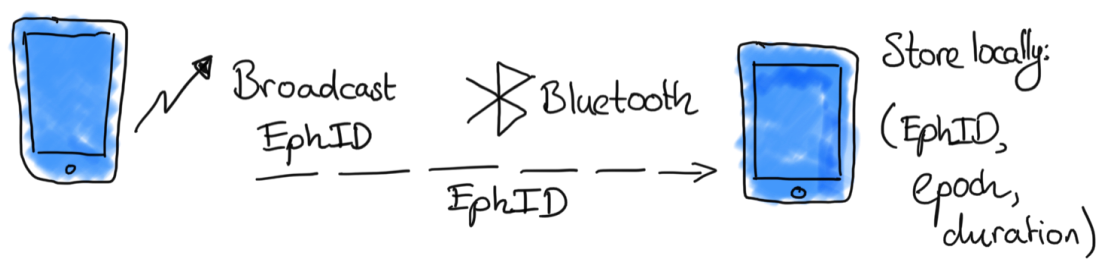
\includegraphics[scale=0.4]{fig/ZZ}
\caption{Processing and storing of observed \texttt{EphID}s.}
\label{ZZ}
\end{figure}
\subsubsection{Proximity tracing}
The proximity tracing process is executed by the backend after a diagnosed patient has
made available to the backend their list of observations [(\texttt{EphID}, epoch, duration)] for the relevant period of time. The backend recovers the long-term pseudo-identifiers of the at-risk users from the reported observed \texttt{EphID}s and triggers a process to identify them. See Figure \ref{ZY}.
\begin{figure}[H]
\centering
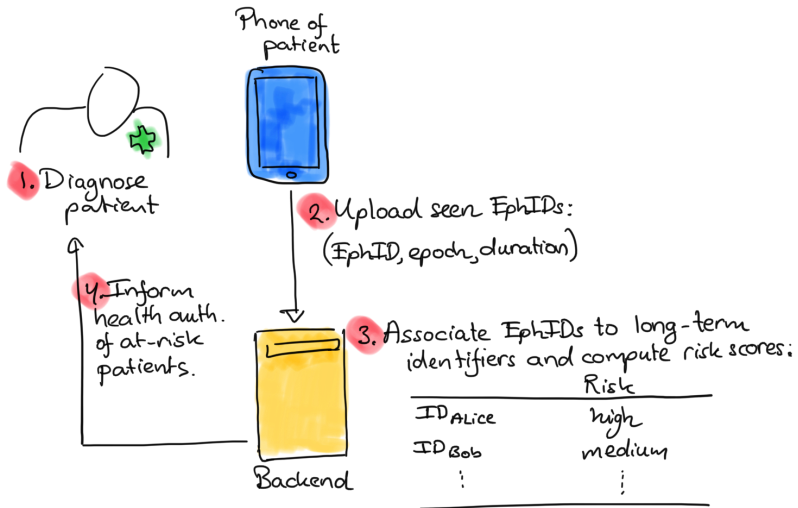
\includegraphics[scale=0.55]{fig/ZY}
\caption{proximity tracing for centralized design}
\label{ZY}
\end{figure}
\subsubsection{Interoperability}
Because \texttt{EphID}s are generated by the backend, if there exist more than one backend (e.g., one backend per country), each backend can only recover their own long term
pseudo-identifiers. Therefore, if infected people have spent time in another country during the infectious period, the backend will receive observed \texttt{EphID}s collected in that country that it cannot interpret. This means that the centralized design requires a “routing” mechanism to ensure that \texttt{EphID}s arrive at the backends that can interpret them. Options to achieve this goal can be to include a country code in the \texttt{EphID} , or to broadcast non-interpretable \texttt{EphID}s  to all other backends to make sure that it reaches home.
\subsubsection{Sharing data with epidemiologists}
In the centralized design, the smartphones never learn which contact events correspond to
contact events with infected individuals, and therefore cannot provide the relevant
information to epidemiologists. To provide this service, the central server must keep all
relevant information and share it with researchers.
\subsubsection{Privacy Comparison}
\textbf{Interaction graph}. The centralized system reveals the interaction graph of each infected user to the backend server. This is by design, as the server maps each time-stamped ephemeral identifier back to a permanent pseudonym to enable contact tracing. The subset of the full interaction graph learned by the server grows quickly as every newly infected user uploads their entire contact history, which can be linked to existing nodes in the graph. Even though the nodes in the graph are pseudonymous, this is a serious privacy concern because graph data is easy to reidentify.

\textbf{Proximity graph}. While in the decentralized design, the proximity graph is only selectively revealed to researchers, the centralised design allows the backend server to learn this information as well. This violates the privacy requirement about limiting inference to minimum necessary and to authorised entities only.

\textbf{Location traceability}. The decentralized design limits the potential for location tracking to infected users over the course of the infectious period. In the centralised system, access to server-side keys (e.g., the backend itself or law enforcement) enables linking ephemeral \texttt{EphID}s to the corresponding permanent app identifier and thus tracing/identifying people based on \texttt{EphID}s  observed in the past, as well as tracing people’s future movements.

\textbf{At-risk individuals}. In the centralized design, by design the backend recovers the identity of the at-risk individuals to be able to notify the health provider about the fact that they are at risk. The health authority will naturally also learn their identities as they need to be contacted. The epidemiologists learn the same information than in the decentralized approach, and so does the eavesdropper that can monitor the exchange of the phone during at-risk notification.

\textbf{Infected individuals}. The centralised and decentralised contact tracing systems share the
inherent privacy limitation that they can be exploited by an eavesdropper to learn whether an individual user got infected and by a tech-savvy user to reveal which individuals in their contact list might be infected now. However, the centralised design does not allow proactive and retroactive linkage attacks by tech-savvy users to learn which contacts are infected because the server never reveals the \texttt{EphID}s of infected users.

\subsubsection{Security Comparison}
\textbf{Fake contact events}. Creating fake at-risk events is easy in the centralised design and can be done retroactively by any tech-savvy infected patient. It does not require broadcasting. It suffices with adding the target \texttt{EphID}s to the list of observed events prior to uploading it to the backend.

\textbf{Suppressing at-risk contacts}. Hiding at-risk contacts is possible in any proximity tracing system.

\textbf{Prevent contact discovery}. Any proximity tracing system based on Bluetooth low energy is susceptible to jamming attacks by active adversaries.
\begin{table}[H]
\centering

\begin{tabular}{p{4cm}p{5cm}p{5cm}p{5cm}}\hline
 & \textbf{Decentralised} &  \textbf{Decentralised} & \textbf{centralised} \\
 & \emph{low cost design} &  \emph{unlinkable design} & \emph{} \\
  \hline
 \multicolumn{3}{l}{\textbf{Privacy Concerns (who can learn what)}}\\
 
 \textit{Interaction graph} & - & - &Backend / State-level \\
 
 \textit{Proximity graph} & Epidemiologist &  Epidemiologist & Epidemiologist / Backend / State-level\\
 
\textit{Location tracking} & Tech-savvy user & - & Backend / State-level\\
\small Of infected users & \small During infectious period & Always \small \\

\textit{Location tracking} & Backend/state-level & - & Backend / State-level\\
\small Of non-infected users & & \small Always\\

At-risk individuals & Tech-savvy user / Eavesdropper & Tech-savvy user / Eavesdropper &  Eavesdropper / Backend /\\
 & & State-level\\
\textit{Infected individuals} & Tech-savvy user / Eavesdropper & Tech-savvy user / Eavesdropper &  Tech-savvy user / Eavesdropper\\

\textit{Percentage infected} & Tech-savvy external with & Noise estimate only & state-level\\
\textit{individuals} & antenna &  Tech-savvy with external antenna \\ \hline

\multicolumn{4}{l}{\textbf{Security Concerns}}\\

\textit{Fake contact events} & Yes & Yes & Yes\\
 & \small Physical proximity + amplified broadcast with knowledge of infected EphID &  \small Physical proximity + amplified broadcast with knowledge of infected EphID & \small Infected tech-savvy user / Backend / State level\\
\textit{Suppressing at-risk} & Yes & Yes \\
\textit{contacts} & \small Tech-savvy user (own contacts only) & \small Tech-savvy user (own contacts only) &  Tech-savvy user / Backend / State-level\\
\textit{Prevent contact} & Yes & Yes & Yes \\
\textit{discovery} & \small Tech-savvy user + broadcast & \small Tech-savvy user + broadcast  & \small Tech-savvy user / Backend / State-level\\ \hline
\end{tabular}
\end{table}


\clearpage
\section{Conclusion}
In this whitepaper, we have outlined two decentralized designs to perform proximity tracing in a privacy-preserving manner. A key requirement for both designs is to minimize exposure of private data, limiting privacy leakage. One design results in an extremely lightweight system, and the other provides extra privacy properties at a small increase in bandwidth. We have also provided evaluation criteria to assess the level of privacy provided by any proximity tracing solution.

Our decentralized designs rely on smartphones to locally compute the risk for an individual user to have contracted the virus based on exposure to infected people. Data about specific contact events, i.e. interactions between individuals, always remains on users’ phones and risk calculation happens locally, according to the guidelines set by the health authorities. In addition, users may voluntarily and privately share data about interactions with infected people (but never contact events itself) with epidemiologists to aid the investigation into the spread of SARS-CoV-2. The decentralised design gives users fine-grained control over the information they share and all data sharing happens under the user’s explicit permission.

We have presented criteria for the evaluation of security and privacy aspects of proximity tracing and have thoroughly evaluated our decentralized designs. Both designs scale to a large number of users with minimal local computation and minimal centralization. Compared to a central design in which the backend would compute risks and inform users, our design protects interaction graphs from the backend, and only a determined tech-savvy adversary can learn any extra information besides the one made visible by the app. The centralized system, in comparison, leaks a lot of unnecessary information about contacts to the backend, and requires large amounts of trust in a central entity.

We strongly urge governments, health authorities, and researchers that any deployment of proximity tracing follows a decentralized design similar to our system to avoid the creation of centralized systems that  have the potential to become surveillance infrastructures.  We are currently working on a reference implementation of the decentralized design which will be released openly during the next weeks.
\end{document}